\problemname{Indoor Orientation}
\noindent
A rapidly growing sport is \emph{indoor orienteering}, where the largest competitions attract
thousands of participants running around places like a campus. Through the organizers' carefully
planned barriers, it becomes a labyrinthine challenge to navigate between control points. Often,
it is essential to optimize the use of stairs, and this is what we will focus on in this task.
Given a map divided into $N$ \emph{areas}, you are to calculate the minimal number of stair runs
the orienteer needs to make to visit the $N$ areas in sequence (to reach a control point in each).

The building contains several vertical stairwells labeled with letters. Each area is located on
a certain floor and is connected to one or more stairwells. A stairwell does not need to be
connected to an area on every floor. For example, stairwell B can connect an area on floor $1$
with another area on floor $3$, without being connected to any area on the intermediate floor $2$.
Moving one floor up or down in a stairwell costs one time unit. However, we do not care about the
time it takes to move within an area and find the control point.

\section*{Input}
The first line contains the integer $N$ ($3\le N \le 15$), the number of areas.

The next $N$ lines each describe one area.
Each line starts with the floor that the area is located at (an integer between $1$ and $100$), 
followed by a string with at least one letter, each letter being chosen from \texttt{A-Z},
which describes the stairwells the floor is connected to.


\section*{Output}
Print an integers: the minimal time required to visit all the $N$ areas in the order given in the input, 
starting in area $1$ and ending in area $N$.


\section*{Points}
Your solution will be tested on several test case groups.
To get the points for a group, it must pass all the test cases in the group.

\noindent
\begin{tabular}{| l | l | p{12cm} |}
  \hline
  \textbf{Group} & \textbf{Point value} & \textbf{Constraints} \\ \hline
  $1$    & $20$      & All strings area a single A. \\ \hline
  $2$    & $80$      & No additional constraints. \\ \hline
\end{tabular}

\section*{Explanation of samples}
\begin{figure}[h]
  \centering
  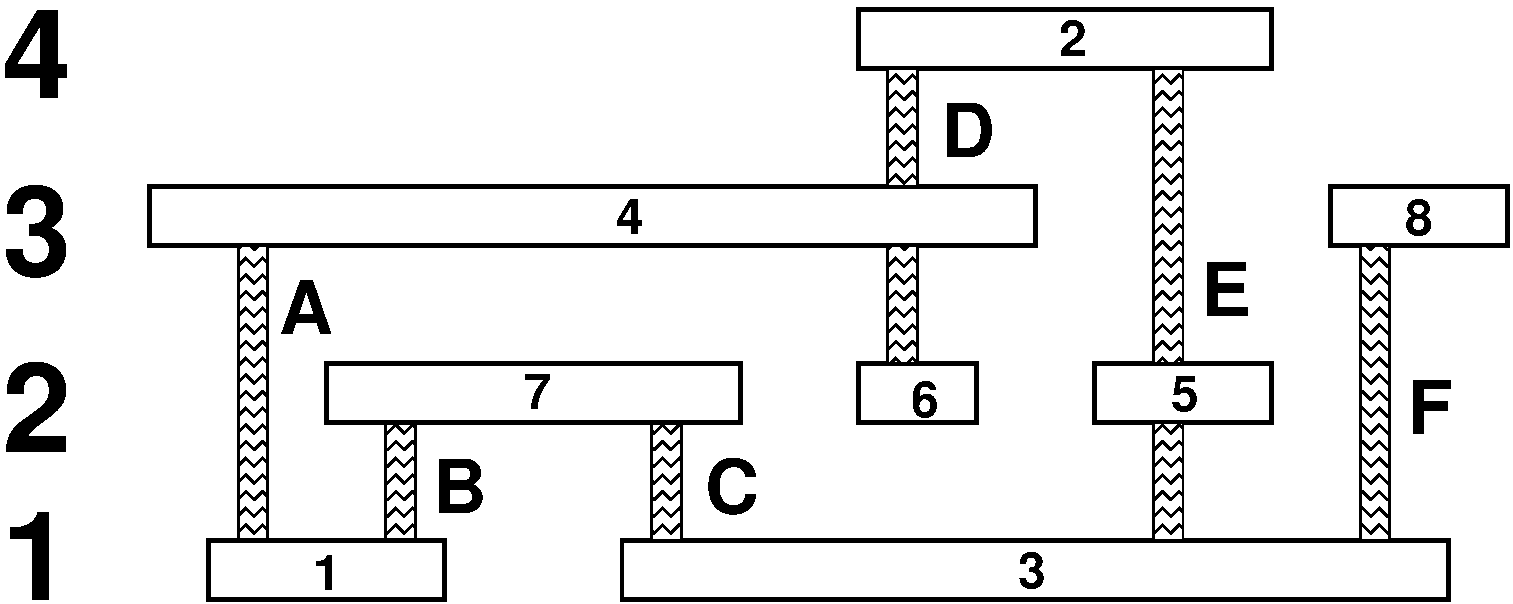
\includegraphics[width=0.6\textwidth]{orient.pdf}
  \caption{
    Cross-section of the building in example 2.
    The large numbers indicate floor numbers, and the small ones indicate the numbering of the areas. One possible shortest path through the entire course is:\\
  }
\end{figure}
In the second example, there is a path with 24 steps: AAD -- EEE -- CBAA -- DEE -- EEDD -- DAAB -- CFF (the letters indicate which staircase was used at each step).
